\documentclass[10pt]{article}
\usepackage[utf8]{inputenc}
\usepackage[english]{babel}
\usepackage{amsmath}
\usepackage{amsfonts}
\usepackage{amssymb}
\usepackage{graphicx}
\usepackage[]{mdframed, caption}
\graphicspath{ {./img/} }

\usepackage{lmodern}
\usepackage{makecell}
\usepackage{hyperref}
\usepackage{listings}
\usepackage{xcolor}

\definecolor{codegreen}{rgb}{0,0.6,0}
\definecolor{codegray}{rgb}{0.5,0.5,0.5}
\definecolor{codepurple}{rgb}{0.58,0,0.82}
\definecolor{backcolour}{rgb}{0.95,0.95,0.92}

\lstdefinestyle{mystyle}{
	backgroundcolor=\color{backcolour},   
	commentstyle=\color{codegreen},
	keywordstyle=\color{magenta},
	numberstyle=\tiny\color{codegray},
	stringstyle=\color{codepurple},
	basicstyle=\ttfamily\footnotesize,
	breakatwhitespace=false,         
	breaklines=true,                 
	captionpos=b,                    
	keepspaces=true,                 
	numbers=left,                    
	numbersep=5pt,                  
	showspaces=false,                
	showstringspaces=false,
	showtabs=false,                  
	tabsize=2
}
\lstset{style=mystyle}
\setcounter{secnumdepth}{3}

\author{Fabio Pavesi}
\title{EDI Client}

\usepackage{titlesec}

\setcounter{secnumdepth}{4}
\titleformat{\paragraph}
{\normalfont\normalsize\bfseries}{\theparagraph}{1em}{}
\titlespacing*{\paragraph}
{0pt}{3.25ex plus 1ex minus .2ex}{1.5ex plus .2ex}

\begin{document}
\maketitle
\newpage
\tableofcontents
\newpage

	\section{Introduction}
		EDI is a template-based metadata editor.
	\section{Templates}
	Templates define the rules for the standards the metadatum it represents must comply to.
	
	Every template must contain x sections:
	
	• settings
	
	• endpointTypes
	
	• datasources
	
	• group
	
	\subsection{Settings}
	
	\subsubsection{userInterfaceLanguage}
	
	Labels can be defined in as many languages as required, by using the \textit{xml:lang} attribute.
	
	The userInterfaceLanguage tag defines which \textit{xml:lang} value should be selected for labels and help tooltips.
	
	\subsubsection{metadataLanguage}
	
	Defines the language to be used when retrieving datasets from datasources.
	
	\subsubsection{metadataEndpoint}
	Defines the endpoint of the EDI Server instance that should be used to convert the metadata into its XML format.
	
	\subsubsection{sparqlEndpoint}
	Defines the default SparQL endpoint.
	
	\subsubsection{requiresValidation}
	Can be set to false (default is true), if you want the metadata to be sent even if they have some errors.
	
	\subsubsection{baseDocument}
	This is, as the name suggests, the base of the XML document to be generated: it is a CDATA and it must include the root element, along with any namespaces that need to be defined.
	
	\subsection{endpointTypes}
	Contains one or more endpointType tags.
	Each tag defines the interface to communicate with a SparQL endpoint.
	
	It must have these attributes:
	\begin{center}
		\begin{tabular}{ | p{0.2\textwidth} | p{0.7\textwidth} | }
			\hline
			Attribute & Description \\ 
			\hline
			xml:id & virtuoso or fuseki \\  
			\hline
			method & GET or POST \\
			\hline
			query & name of the parameter holding the query \\
			\hline
		\end{tabular}
	\end{center}
	
	And the child tag \textit{parameters}, whose children are \textit{parameter} tags.
	Each parameter defines a query-string parameter with name and value to be sent to the endpoint.
	
	Name and value are specified as attributes of the \textit{parameter} tags.
	
	\subsection{datasources}
	Datasources provide valid values for specific \textit{items}.
	
	A collection of datasources: each datasource can be one of \textit{codelist}, \textit{sparql} or \textit{singleton}.
	
	\subsubsection{sparql}
	The most general type of datasource is a SparQL query.
	
	It has two attributes:
	\begin{center}
		\begin{tabular}{ | p{0.2\textwidth} | p{0.7\textwidth} | }
			\hline
			Attribute & Description \\ 
			\hline
			xml:id & unique id \\  
			\hline
			endpointType & reference to an existing (declared) endpointType \\
			\hline
		\end{tabular}
	\end{center}

	It requires one child tag named \textit{query}, specifying the SparQL query.
	
	Query can include a \textit{\$search\_param} token, which, if found, will be given a value based, for example, on user text.
	
	\subsubsection{codelist}
	A codelist is a simplified version of a \textit{sparql} datasource, based on a pre-defined query, accessed via its URI, specified by the child tag \textit{uri}.
	
	\subsubsection{singleton}
	\label{singleton}
	A singleton is a special stateful \textit{sparql} datasource guaranteed to have only a single instance, so that it can be used to keep some items aligned to some other item whenever the latter changes.
	
	The item triggering said alignment is specified by the attribute \textit{triggerItem}.
	
	Another datasource is always needed, for the singleton to work: the trigger item refers to a sparql or codelist datasource, whereas the dependent items are connected to it via the singleton, which will refresh and select a single row of the singleton dataset, which is linked, in turn, to the uri of the row selected by the trigger item.
	
	
	\subsection{group}
	This section defines the form's structure in terms of its base components: \textbf{group}s, \textbf{element}s and \textbf{item}s.
	
	Groups hold elements (see \ref{element}) which, in turn, contain items (see \ref{item}).
	Each group must have an \textit{xml:id} and it can have a label for every language it should support.
	
	A template will be composed by one or more groups.
	
	Attributes:
	\begin{center}
		\begin{tabular}{ | p{0.2\textwidth} | p{0.7\textwidth} | }
			\hline
			Attribute & Description \\ 
			\hline
			xml:id & unique id \\
			\hline
		\end{tabular}
	\end{center}
	
	Child tags:
	\begin{center}
		\begin{tabular}{ | p{0.2\textwidth} | p{0.7\textwidth} | }
			\hline
			Tag & Description \\ 
			\hline
			label & one for each xml:lang to be supported \\
			help & one for each xml:lang to be supported \\
			\hline
			element & one for each element \\
			\hline
			
		\end{tabular}
	\end{center}
	
	\begin{figure}[h]
		\caption{Group example}
		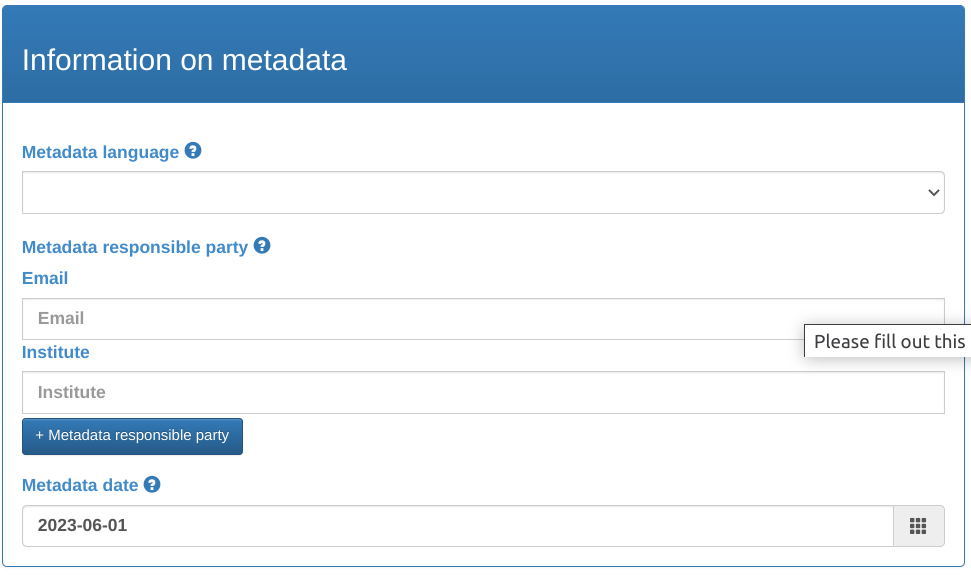
\includegraphics[width=10cm]{Group example.png}
		\centering
	\end{figure}
	
	\begin{lstlisting}[language=xml]
		<group xml:id="info_md">
			<label xml:lang="en">Information on metadata</label>
			<label xml:lang="it">Informazioni sui metadati</label>
		...
		</group>
	\end{lstlisting}
	
	\subsubsection{element} \label{element}
	Elements are groupings of *item*s that share conceptual purpose and a shared root in the resulting XML.
	
	Attributes:
		\begin{center}
		\begin{tabular}{ | p{0.2\textwidth} | p{0.7\textwidth} | }
			\hline
			Attribute & Description \\ 
			\hline
			xml:id & unique id \\
			\hline
			isMandatory & \textbf{true} if all underlying items must have a value \\ & \textbf{false} otherwise \\
			\hline
			isMultiple & \textbf{true} if element can have multiple instances \\ & \textbf{false} otherwise  \\
			\hline
			alternativeTo & if present it means this element is an exclusive alternative for another item: only the one of the two that has been filled in will make it to the final XML \\
			\hline
		\end{tabular}
	\end{center}
	
		Child tags:
	\begin{center}
		\begin{tabular}{ | p{0.2\textwidth} | p{0.7\textwidth} | }
			\hline
			Tag & Description \\ 
			\hline
			label & one for each xml:lang to be supported \\
			help & one for each xml:lang to be supported \\
			\hline
			hasRoot & represents the root tag in the destination XML \\
			\hline
			produces & container tag for \textit{items} \\
			\hline
			
		\end{tabular}
	\end{center}
	
	\begin{figure}[h]
		\caption{Element example (single item)}
		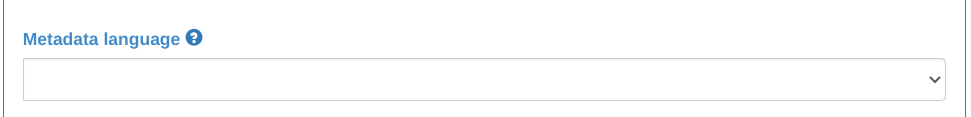
\includegraphics[width=10cm]{Element single item.png}
		\centering
	\end{figure}
	
	\begin{lstlisting}[language=XML]
		<element xml:id="id_md" isMandatory="true" isMultiple="false">
			<label xml:lang="en">File identifier</label>
			<label xml:lang="it">Identificatore del file</label>
			<help xml:lang="en">The element must contain, as a prefix, the iPA code assigned by 
			the Administration in the Index of Public Administrations (e.g., "cnr:112358").</help>
			<help xml:lang="it">L'elemento deve contenere, come prefisso, il codice iPA assegnato
			all'Amministrazione nel momento dell'accreditamento all'Indice delle Pubbliche
			Amministrazioni (es. "cnr:112358").</help>
			<hasRoot>/gmd:MD_Metadata/gmd:fileIdentifier</hasRoot>
			<produces>
				<item hasIndex="1" xml:id="id_md_1" queryStringParameter="uid" isFixed="true" hasDatatype="string">
				<hasPath>/gmd:MD_Metadata/gmd:fileIdentifier/gco:CharacterString</hasPath>
				</item>
			</produces>
		</element>
	\end{lstlisting}
	
	\begin{figure}[h]
		\caption{Element example (multiple items)}
		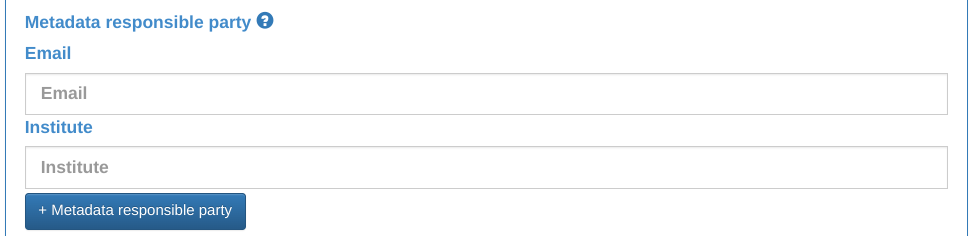
\includegraphics[width=10cm]{Element multiple items.png}
		\centering
	\end{figure}
	
	
	\paragraph{item} \label{item}
	
	Attributes:
\begin{center}
	\begin{tabular}{ | p{0.3\textwidth} | p{0.6\textwidth} | }
		\hline
		Attribute & Description \\ 
		\hline
		xml:id & unique id \\
		\hline
		hasIndex & a string representing the index of this item in the order of shown items inside the element \\
		\hline
		outIndex & a string representing the index of this item in the order required inside the element XML representation \\
		\hline
		hasDatatype & data type of the item: must be one of the \hyperref[datatypes]{suupported data types} \\
		\hline
		isFixed & \textbf{true}: the item is neither visible nor editable \\
		& \textbf{false}: the item is visible and editable \\
		\hline
		hasPath & the destination path in the XML output document: it can be relative relative to the hasRoot attribute of containing element \\
		\hline
		datasource & optional datasource id holding allowed values \\
		\hline
		field & optional field holding the allowed value \\
				\hline
		isLanguageNeutral & optional indication to instruct EDI Client to use language neutral results from a datasource, overriding the default metadata language \\
		\hline
		defaultValue & optionally used to 		specify a default value for the item \\
		\hline
		useCode & optionally specifies that the code (URI or urn) field should be used from the datasource \\
		\hline
		show & (\textbf{TODO: check if really implemented}) optionally override default control used as input with a specific one \\
		\hline
		queryStringParameter & if specified, it allows the initial value of this item to be specified in the query string: the value of this attribute defines the key / value pair in the query string \\
		\hline
	\end{tabular}
\end{center}

Child tags:
\begin{center}
	\begin{tabular}{ | p{0.2\textwidth} | p{0.7\textwidth} | }
		\hline
		Tag & Description \\ 
		\hline
		label & one for each xml:lang to be supported \\
		help & one for each xml:lang to be supported \\
		\hline
		hasRoot & represents the root tag in the destination XML \\
		\hline
		produces & container tag for \textit{items} \\
		\hline
		
	\end{tabular}
\end{center}

\section{Data Types} 
\label{datatypes}

\subsection{Base data types}
\label{base-types}

\subsubsection{text}
\label{text}

\begin{figure}[h]
	\caption{Text example}
	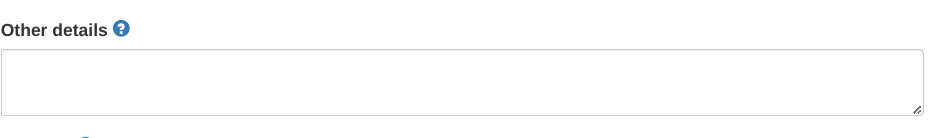
\includegraphics[width=10cm]{Textarea.png}
	\centering
\end{figure}

\subsubsection{string}
\label{string}

Simplest control type: a small rectangle accepting generic text.

\subsubsection{URN}
\label{URN}

Calculated by the server if \textbf{isFixed="true"}.
Server will generate a valid and unique URN for you.

\subsubsection{URI}
\label{URI}

Accepts a string and verifies it's an URI.

\subsubsection{URL}
\label{URL}
Accepts a string and verifies it's an URL.

\subsubsection{int}
\label{int}
Accepts a string and verifies it's an only contains numeric digits.

\subsubsection{float}
\label{real}

Accepts a string and verifies it's an only contains numeric digits or the decimal separator (i.e. a dot).

\begin{mdframed}
	With attribute \textbf{show="sliderfloat"}
	
	Shows a slider with a minimum and a maximum value and the position generates a value for this control.
	
	\begin{lstlisting}[language=xml]
		<item hasDatatype="float" show="sliderfloat" hasIndex="4" xml:id="slider2" isFixed="false" min="0.0" max="100.00" step="0.5">
		<label xml:lang="en">Slider Float 2</label>
		<label xml:lang="it">Slider Float 2</label>
		<defaultValue>49</defaultValue>
		<hasValue>70</hasValue>
		<hasPath>slider</hasPath>
		</item>
	\end{lstlisting}
	
	
	{\centering
		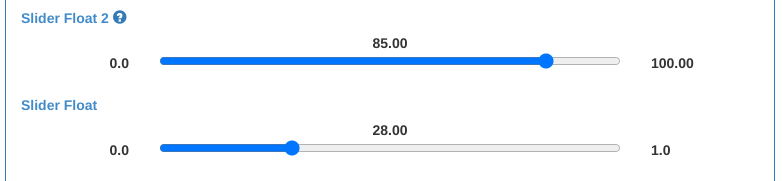
\includegraphics[width=10cm]{FloatSlider.png}
		\captionof{figure}{Example of floating-point control with sliderfloat}
		\par
	}
	
	
\end{mdframed}


Shows a slider with a minimum and a maximum value and the position generates a value for this control.

\begin{lstlisting}[language=xml]
	<item hasDatatype="float" show="sliderfloat" hasIndex="4" xml:id="slider2" isFixed="false" min="0.0" max="100.00" step="0.5">
	<label xml:lang="en">Slider Float 2</label>
	<label xml:lang="it">Slider Float 2</label>
	<defaultValue>49</defaultValue>
	<hasValue>70</hasValue>
	<hasPath>slider</hasPath>
	</item>
\end{lstlisting}


\subsubsection{real}
\label{double}

Same as \textit{float}.

\subsubsection{double}
\label{double}

Same as \textit{float}.


\subsubsection{codelist}
\label{codelist}

\begin{lstlisting}[language=xml]
 <item hasIndex="1" xml:id="ling_md_1" isLanguageNeutral="true" isFixed="false" hasDatatype="codelist" datasource="languages" show="combobox">
	<hasPath>/gmd:MD_Metadata/gmd:language/gmd:LanguageCode</hasPath>
</item>
\end{lstlisting}
\begin{figure}[h]
	\caption{Codelist example with \textit{show="combobox"}}
	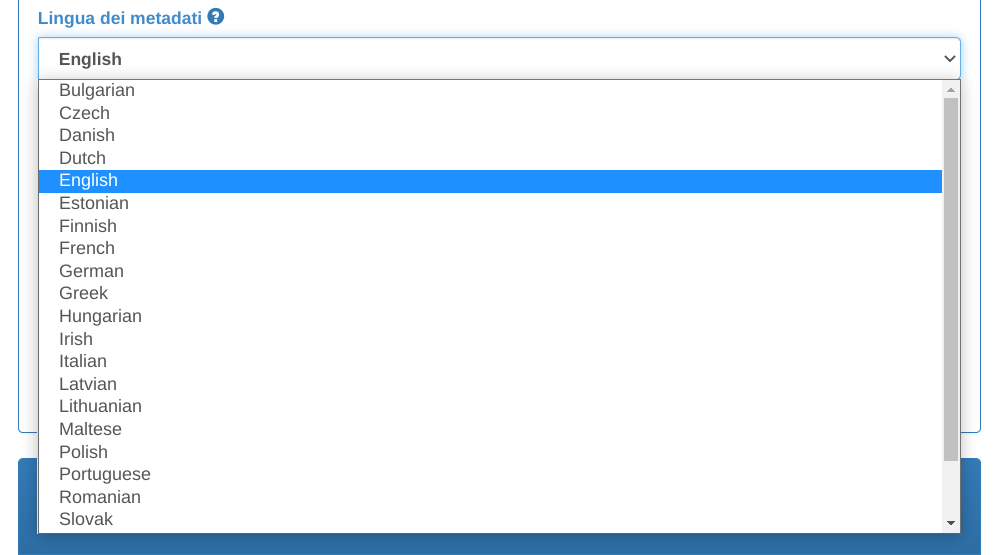
\includegraphics[width=10cm]{Codelist.png}
	\centering
\end{figure}

\subsubsection{autoCompletion}
\label{autoCompletion}

Similar to a \textit{codelist}, but preferrable with datasources containing many rows.

A textbox querying the datasource associated to the control for matching values.
Starts querying when at least 3 characters are entered.

\begin{lstlisting}[language=xml]
	<item hasIndex="1" xml:id="md_resp_1" outIndex="2" isFixed="false" hasDatatype="autoCompletion" datasource="person">
		<label xml:lang="en">Email</label>
		<label xml:lang="it">Email</label>
			<hasPath>/gmd:MD_Metadata/gmd:contact/gmd:CI_ResponsibleParty/gmd:contactInfo/gmd:CI_Contact/gmd:address/gmd:CI_Address/gmd:electronicMailAddress/gco:CharacterString</hasPath>
	</item>
\end{lstlisting}
\begin{figure}[h]
	\caption{AutoCompletion example}
	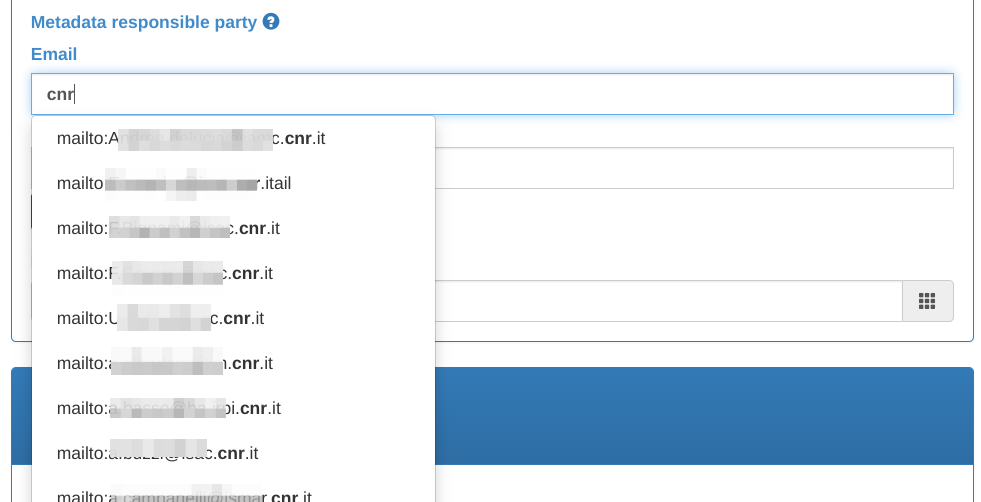
\includegraphics[width=10cm]{Autocompletion.png}
	\centering
\end{figure}


\subsubsection{boolean}
\label{boolean}

Shows a check-box, thus allowing only values \textbf{true} or \textbf{false}.


\subsection{Special case data types}
\subsubsection{label}
\label{label}

Shows read-only text.

\subsubsection{image}
\label{image}

Given an URL pointing to a valid image in the value, it shows the image.

\subsubsection{qrcode}
\label{qrcode}

Shows whatever the value is as a QR code.


\subsubsection{select}
\label{select}

The select datatype signifies that the item's value is based on some selection occurring in another item called a \textit{trigger item}.

It must be based on a data source of type \textbf{singleton} (see \ref{singleton}).

Sometimes the trigger item can be based on the same data source as its connected \textit{select} items, but it can be based on its own data source.

Each \textit{select} item must declare the field it represents in the datasouce.

\begin{lstlisting}[language=xml]
	<item hasIndex="2" xml:id="resp_2" outIndex="1" field="inst" isFixed="false" hasDatatype="select" datasource="personS_2">
		<label xml:lang="en">Institute</label>
		<label xml:lang="it">Ente</label>
		<hasPath>/gmd:MD_Metadata/gmd:identificationInfo/gmd:MD_DataIdentification/gmd:citation/gmd:CI_Citation/gmd:citedResponsibleParty/gmd:CI_ResponsibleParty/gmd:organisationName/gco:CharacterString</hasPath>
	</item>
\end{lstlisting}

\subsubsection{copy}
\label{copy}

\begin{figure}[h]
	\caption{String example, in this case it is part of a \textit{isMultiple="true"} element, as you can tell from the "+" button underneath it}
	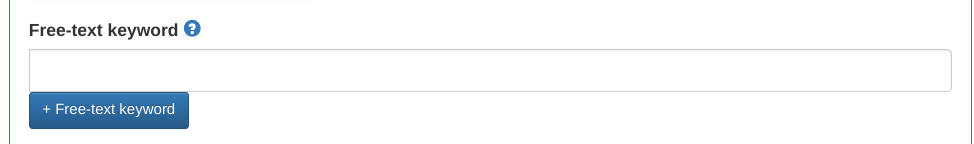
\includegraphics[width=10cm]{String.png}
	\centering
\end{figure}


% \subsubsection{dependent}
% \label{dependent}

\subsubsection{function}
\label{function}

Special data type.
Its value is calculated by the server by using its template \textit{hasValue} as an XPath run \textbf{against the parts of document that have already been generated}.

\subsubsection{ref}
\label{ref}

Special data type.
In the generated metadata document, it copies the Xpath specified in the \textit{hasValue} attribute to the Xpath specified by the \textit{hasPath} attribute.

\begin{lstlisting}[language=xml]
<item hasDatatype="ref" hasIndex="7" xml:id="title_7" isFixed="true">
	<hasPath>dct:description/@xml:lang</hasPath>
	<hasValue>/rdf:RDF/dcatapit:Dataset/dct:title/@xml:lang</hasValue>
</item>
\end{lstlisting}

In the example above, once the XML document is fully written, the \textbf{xml:lang} attribute of \textbf{dct:description} is set to equal the same attribute in \textbf{/rdf:RDF/dcatapit:Dataset/dct:title}.

\subsubsection{autonumber}
\label{autonumber}

Represents a value that's incremented every time it is encountered within the containing element.

Value is assigned by EDI Server.

\subsubsection{hidden}
\label{hidden}

Hidden item: it is \textit{fixed} by default (i.e. read-only).

\subsubsection{date}
\label{date}

Requests a date from the user, via a small calendar.

Requires a \textit{defaultValue}, which can be the macro \textit{\$TODAY\$}.

\begin{lstlisting}[language=xml]

<item hasDatatype="date" hasIndex="7" xml:id="test_7" isFixed="false">
	<label xml:lang="en">Issues date</label>
	<label xml:lang="it">Data di rilascio</label>
	<help xml:lang="en">Help</help>
	<help xml:lang="it">Help</help>
	<hasValue>dct:issued</hasValue>
	<defaultValue>$TODAY$</defaultValue>
</item>

\end{lstlisting}

\begin{figure}[h]
	\caption{Date example}
	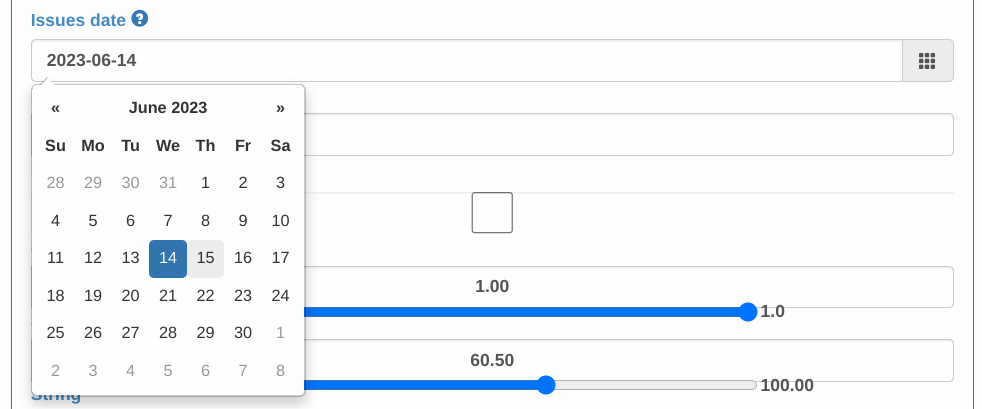
\includegraphics[width=10cm]{Date.png}
	\centering
\end{figure}


\subsubsection{dateRange}
\label{dateRange}

Same as \textit{date}, except that it requests a start and an end date.

\begin{lstlisting}[language=xml]
	
<item hasIndex="8" xml:id="est_temp_8" isFixed="false" hasDatatype="dateRange">
	<label xml:lang="en">Start date</label>
	<label xml:lang="it">Data inizio</label>
	<start>
		<label xml:lang="en">Start date</label>
		<label xml:lang="it">Data inizio</label>
		<hasPath>/gmd:MD_Metadata/gmd:identificationInfo/gmd:MD_DataIdentification/gmd:extent/gmd:EX_Extent/gmd:temporalElement/gmd:EX_TemporalExtent/gmd:extent/gml:TimePeriod/gml:beginPosition</hasPath>
	</start>
	<end>
		<label xml:lang="en">End date</label>
		<label xml:lang="it">Data fine</label>
		<hasPath>/gmd:MD_Metadata/gmd:identificationInfo/gmd:MD_DataIdentification/gmd:extent/gmd:EX_Extent/gmd:temporalElement/gmd:EX_TemporalExtent/gmd:extent/gml:TimePeriod/gml:endPosition</hasPath>
	</end>
</item>
	
\end{lstlisting}



\subsubsection{boundingBox}
\label{boundingBox}

Requests a geographic bounding box from the user.
It can be specified either by inputting the coordinates in 4 text boxes, or by drawing a rectangle on a map.

\begin{lstlisting}[language=xml]
	
<item hasIndex="1" xml:id="loc_geo_1" isFixed="false" hasDatatype="boundingBox">
	<westLongitude outIndex="1" queryStringParameter="westlon">
		<label xml:lang="en">W longitude</label>
		<label xml:lang="it">Longitudine O</label>
		<hasPath>/gmd:MD_Metadata/gmd:identificationInfo/gmd:MD_DataIdentification/gmd:extent/gmd:EX_Extent/gmd:geographicElement/gmd:EX_GeographicBoundingBox/gmd:westBoundLongitude/gco:Decimal</hasPath>
	</westLongitude>
	<eastLongitude outIndex="2" queryStringParameter="eastlon">
		<label xml:lang="en">E longitude</label>
		<label xml:lang="it">Longitudine E</label>
		<hasPath>/gmd:MD_Metadata/gmd:identificationInfo/gmd:MD_DataIdentification/gmd:extent/gmd:EX_Extent/gmd:geographicElement/gmd:EX_GeographicBoundingBox/gmd:eastBoundLongitude/gco:Decimal</hasPath>
	</eastLongitude>
	<northLatitude outIndex="4" queryStringParameter="northlat">
		<label xml:lang="en">N latitude</label>
		<label xml:lang="it">Latitudine N</label>
		<hasPath>/gmd:MD_Metadata/gmd:identificationInfo/gmd:MD_DataIdentification/gmd:extent/gmd:EX_Extent/gmd:geographicElement/gmd:EX_GeographicBoundingBox/gmd:northBoundLatitude/gco:Decimal</hasPath>
	</northLatitude>
	<southLatitude outIndex="3" queryStringParameter="southlat">
		<label xml:lang="en">S latitude</label>
		<label xml:lang="it">Latitudine S</label>
		<hasPath>/gmd:MD_Metadata/gmd:identificationInfo/gmd:MD_DataIdentification/gmd:extent/gmd:EX_Extent/gmd:geographicElement/gmd:EX_GeographicBoundingBox/gmd:southBoundLatitude/gco:Decimal</hasPath>
	</southLatitude>
</item>	
\end{lstlisting}

\begin{figure}[h]
	\caption{Bounding box example}
	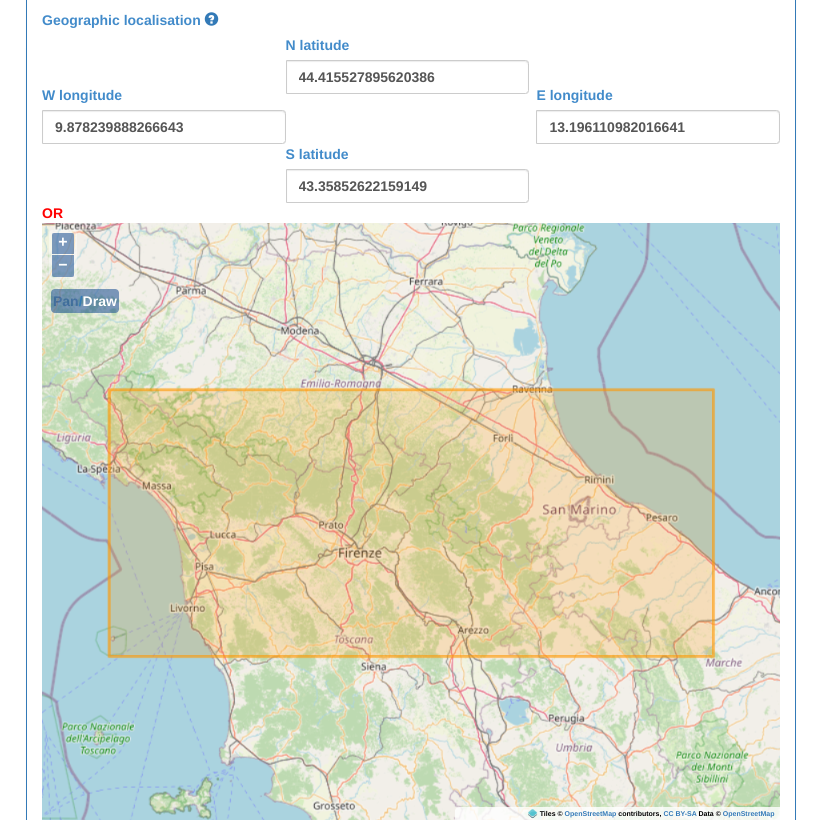
\includegraphics[width=10cm]{BoundingBox.png}
	\centering
\end{figure}	


\end{document}\documentclass[10pt,a4paper]{article}
